\documentclass{article}
\usepackage[english]{babel}
\usepackage[utf8]{inputenc}
\usepackage{xcolor}
\usepackage[pdftex]{graphicx}
\usepackage{listings}
\usepackage{amsmath}
\usepackage[a4paper,includeheadfoot,margin=2.54cm]{geometry}
\usepackage{amsfonts}
\usepackage{fancyhdr}
\usepackage{titling}
\usepackage{algorithm}
\usepackage{algpseudocode}
\usepackage{hyperref}
\usepackage[export]{adjustbox}
\usepackage{csquotes}
\usepackage{booktabs}
\usepackage{subcaption}
\usepackage{longtable}
\usepackage{makecell}

\pagestyle{fancy}
\fancyhf{}
%\fancyhead[LE,RO]{\theauthor}
\fancyhead[RE,LO]{E4 project : Maximin Affinity Learning of Image Segmentation - Appendix}
\fancyfoot[CE,CO]{\leftmark}
\fancyfoot[LE,RO]{\thepage}

\usepackage[thinlines]{easytable}

\setlength{\parindent}{0ex}


\title{E4 project : Maximin Affinity Learning of Image Segmentation\\Appendix}
\author{Josselin Lefèvre, Maxime Burchi, Maxime Schoenberger}
\date{July 2020}

\begin{document}

\setcounter{tocdepth}{2}
\maketitle
\pagebreak
\tableofcontents
\pagebreak


\section{Introduction}
The goal of this project is to implement Maximin Affinity Learning of Image
Segmentation (or MALIS for short) as introduced in~\cite{turaga_maximin_2009}.
It is a method used to obtain an image segmentation that is mainly used on medical
imagery.\\

\begin{figure}[!htbp]
	\centering
	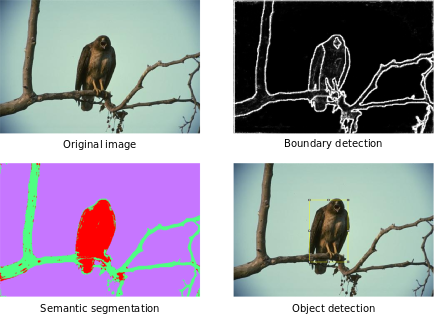
\includegraphics[width=0.7\linewidth]{./images/segmentation.png}
	\caption{Illustration of image segmentation, from
	\href{imagej.net/File:TWS-application-examples.png}{ImageJ}}%
	\label{fig:segmentation}
\end{figure}

As we can see in figure~\ref{fig:segmentation} there are multiple ways to
produce an image segmentation. In the top right corner we can see a boundary
detection of the original image, where borders between objects are in white and
objects are in black. Here we only get the separation between objects but no
information on the objects/segments themselves.\\
In the bottom left corner, we have an example of semantic segmentation of our
image. Here the idea is to classify every pixels in predefined classes (here
red is the bird, green the tree and purple the background). We then obtain a
segmentation with different information, which is not necessarily better than
boundary detection since both solve different problems.\\
On the bottom right corner we have an example of object detection. Even though
it gives us a rough estimate of the structure of the image and the objects
present in it, it is not considered  a segmentation and is a whole other class
of algorithms.\\

In the case of MALIS, we will try to obtain a boundary detection, or what we
could call an edge based segmentation. There are various ways to generate an
image segmentation of this kind, the simplest one being an algorihm such as
Canny's algorithm, or more advanced methods such as watersheds or more recently
neural networks based approaches. The idea with MALIS is to optimize directly a
measure of segmentation quality, which had not been done before. This is a
really interesting idea since segmentations are always evaluated using various
metrics (Rand Index, Variation Of Information ...) and optimizing one directly
could lead to better results, at least for this metric.\\

Our goal in this project is to implement the original MALIS
paper~\cite{turaga_maximin_2009} and also it's improvement
in~\cite{funke_large_2019}.\\

In this report, we will first describe how MALIS works in more details. We will
then look at how we implemented it and some implementation challenges that we
faced. We will then look at the results we have gotten so far, by implementing
the original method. Afterwards, we will look at how the method was improved
and what we will try to implement in the coming semester. Finally we will take
a look at how we worked as a team throughout this project.



%------------------------------------------------------------------------------
%\clearpage

\section{Neural Network Architectures}
\subsection{A Deeper U-Net Mala}

The first network we implemented is a U-Net Mala with a deeper architecture using zero padding for every convolution operation. We tried this experience because a deeper architecture is often associated with deeper meaning representation during learning. A padding for every convolution allows us to stack more layers adding a 5th level with 1024 filters without diminishing the size of the output gradient predictions along height and width.
As previous experiences, the network takes a $256\times256$ input image and output the gradients along $x$ and $y$ axes for the whole image. Convolutional layers with $3\times3$ kernel size and Rectified Linear Unit activations are also used and max pooling operations stay the same.
Bilinear upsampling layers are replaced by transposed convolutions as described in \cite{funke_large_2019}.\\

The network is trained for 230.000 iterations using an Adam optimizer with an initial learning rate $\alpha = 10^{-4}$, $\beta_{1}=0.95$, $\beta_{2}=0.99$ et $\epsilon=10^{-8}$. During inference,  a simple pixel wise mean followed by a threshold is applied to the two gradient volumes to create the final segmentation.\\

With this network, we were able to generate thinner segmentations for every frame and get better results on the Cremi test-set than previous experiences.


\subsection{Multi Input Images}

This architecture came with the idea to use 3 successive frames as input and compute the loss only on the center image in order to predict a better segmentation along the depth. As we know, Cremi is a volume dataset so a network linking a frame to its neighbors should better predict segmentations along the depth than previous networks.\\
This network shares the same architecture as U-Net Mala described in previous works, optimizer and other hyperparameters for training and inference remain the same.\\

\subsection{3D U-Net Mala}

One of our main objective was to implement the network as described in \cite{funke_large_2019}. This part describes the implementation of a 3 dimensional U-Net like architecture for volume segmentation. Mathematical operations and training parameters are the same as described in the paper. The network takes $84\times268\times268$ (depth, height, width) patches as input and predict the gradient along x, y and z axes defined by $56\times56\times56$ outputs.\\

\begin{figure}[!htbp]
	\centering
	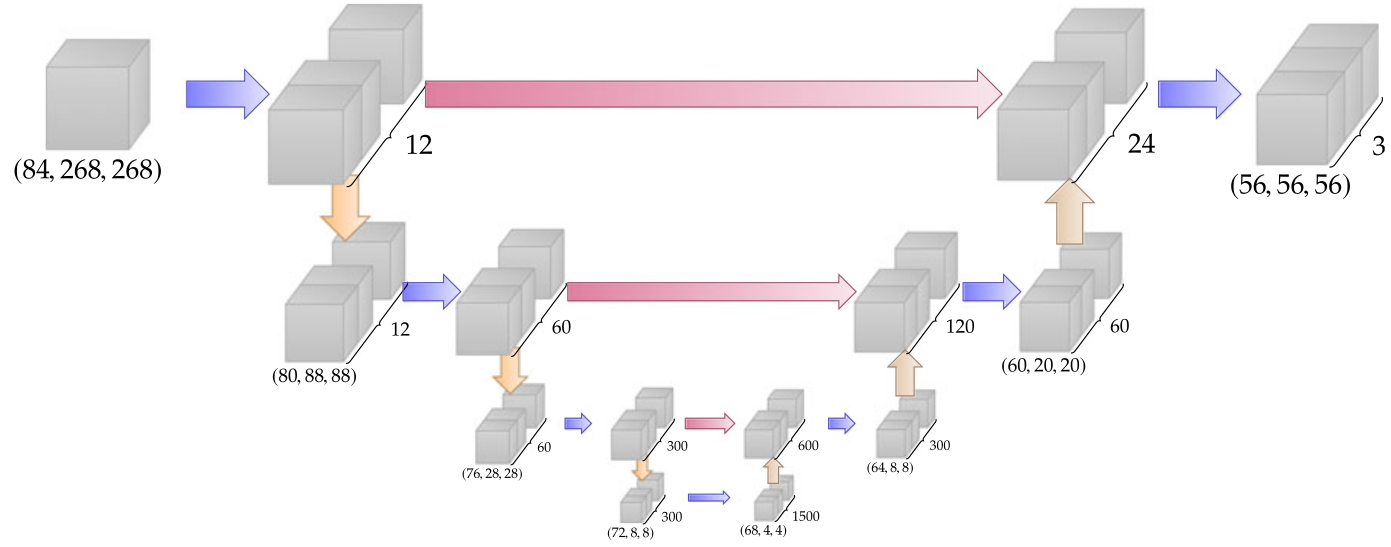
\includegraphics[width=0.8\linewidth]{./images/mala_architecture.png}
	\caption{Overview of the U-Net architecture used for the Cremi dataset in \cite{funke_large_2019}. The network is 4 levels deep and doesn’t use padding for convolution operations. Transposed convolutions and max pooling layers use a stride of 3 along height and width but do not affect the input size along the depth. Relu activations are used after every convolution layer.}%
	\label{fig:mala_unet}
\end{figure}

To implement the network, we created a 3D version of the processing algorithms for calculating edge weights and decompose the dataset into patches. For inference, every patch of the volume is fed into the network, then gradients volumes are reconstructed for the 3 axes.

\begin{figure}[!htbp]
	\centering
	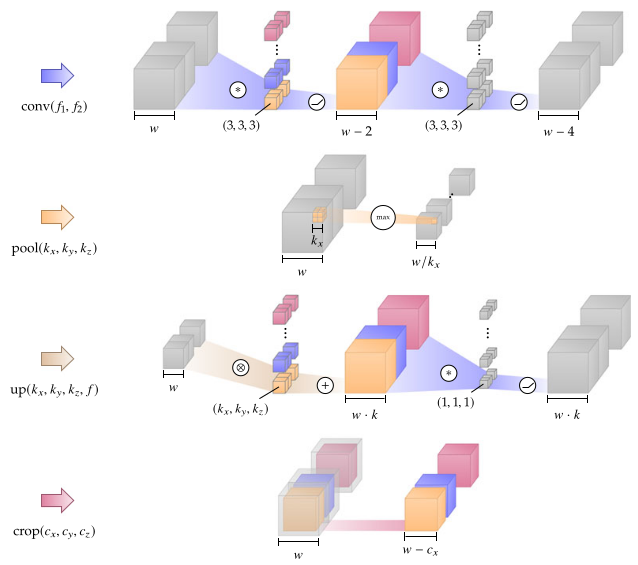
\includegraphics[width=0.8\linewidth]{./images/architecture_details.png}
	\caption{Details of convolution operations (blue), pooling (orange), transpose convolution (brown) and crops (red). Every transpose convolution layer is followed by a concatenation operation between outputs and crops from the same level.  A $1\times1\times1$ convolution follows the concatenation to reduce the filter dimension.}%
	\label{fig:mala_unet}
\end{figure}




%------------------------------------------------------------------------------
%\clearpage

\section{Training observations}
\subsection{Collapsing}

During the training we saw the network collapse several times. The gradients took on a uniform value and the network was unable to get out of this situation. After comparing the losses for each time this happened we were unable to find a pattern. The number of iterations was also quite different: 50K, 60K or 70K iterations.\\

We also checked the predictions before this collapse but we did not see anything that could have alerted us. The only common point is that each time the "grids" which we will talk about in the next part had already appeared.

\subsection{Bad predictions along Z}

As described in section 6.3 of the previous report, we encountered a problem of dissimilarity between the predictions in x and in y. We can note that this inconsistency in the predictions has completely disappeared. However, we were able to see a "grid" appear in the zones corresponding to the darkest zones of the input image such as the nuclei.\\

This phenomenon only occurred after a certain number of iterations and never disappeared.\\

\begin{figure}[!htbp]
    \centering
    \begin{subfigure}[t]{0.31\textwidth}
        \centering
        \frame{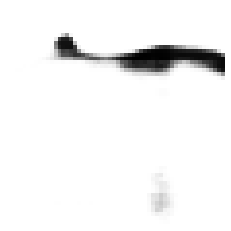
\includegraphics[height=0.7\textwidth]{./images/grad_x.png}}
        \caption{Affinity along the X axis}
    \end{subfigure}%
    ~ 
    \begin{subfigure}[t]{0.31\textwidth}
        \centering
        \frame{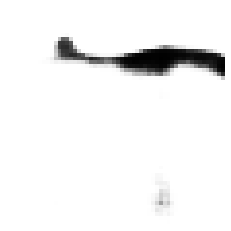
\includegraphics[height=0.7\textwidth]{./images/grad_y.png}}
        \caption{Affinity along the Y axis}
    \end{subfigure}
    ~ 
    \begin{subfigure}[t]{0.31\textwidth}
        \centering
        \frame{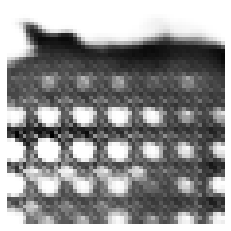
\includegraphics[height=0.7\textwidth]{./images/grid.png}}
        \caption{Affinity along the Z axis}
    \end{subfigure}
	\caption{Bad affinity prediction along the Z axis}
	\label{fig:grid}
\end{figure}

We believe that this is due to the anisotropy of the volumes. In the Cremi dataset the resolution along the $z$ axis is ten times greater than that in $x$ and $y$. It would be interesting to interpolate the frames according in order to reduce this difference and observe if this phenomenon still occurs. Another simpler solution to verify the source of this problem would be to train the network on isotropic volumes like Fib-25.\\

\subsection{Deterioration of the agglomeration}

We worked on the implementation of the agglomeration method proposed in \cite{funke_large_2019} that the first group had carried out in order to optimize it and compare it with that provided by the authors of the paper (a library called \href{https://github.com/funkey/waterz}{waterz}). By computing the region adjacency graph of the regions only once, and not at every step as previously, we have succeeded in reducing the execution time and we have obtained results quite comparable to those obtained with waterz. The differences can be explained by the discretization of the initial costs into k-bins which we have not implemented. But waterz is still much faster than our python implementation\\

As described earlier we saw a "grid" appear in areas corresponding to the the darkest regions of the input. We wondered if this could cause the agglomeration of regions along the z axis to deteriorate.
We then implemented the agglomeration algorithm on different affinities. First those which do not present this grid and then those where it is present. To carry out our experiment, we preferred to take the ground truth as a fragment, taking care to decouple the x-y frames along the z axis by adding to each value of an x-y frame its index.\\

\begin{figure}[!htbp]
    \centering
    \begin{subfigure}[t]{0.31\textwidth}
        \centering
        
\includegraphics[height=1\textwidth]{./images/agglo.png}
    \end{subfigure}%
    ~ 
    \begin{subfigure}[t]{0.31\textwidth}
        \centering
        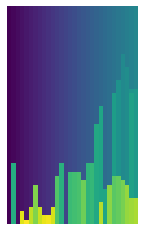
\includegraphics[height=1\textwidth]{./images/bad_agglo.png}
    \end{subfigure}
    ~ 
    \begin{subfigure}[t]{0.31\textwidth}
        \centering
        
\includegraphics[height=1\textwidth]{./images/agglo_gt.png}
    \end{subfigure}
	\caption{On the left the x-z cut from the result of agglomeration on affinities without the grid, at the center x-z cut from the result of agglomeration on affinities with the grid and on the right the ground truth.}
	\label{fig:agglomeration}
\end{figure}

After taking several x-z cuts we could see that the agglomeration according to z suffered from the presence of this grid as we can see in figure~\ref{fig:agglomeration}.

%------------------------------------------------------------------------------
\clearpage

\section{Results}
\subsection{Evaluation method}
We evaluated our method with two different datasets : CREMI and ISBI datasets.\\
Both are composed of Drosophila melanogaster adult brain images.\\

Our 3D image of size X x Y x Z was easier to predict in two-dimension. 
That's why we considered Z images of size X x Y which were stacked together to get back a 3D image.\\
A very simple architecture is used for the training.
It's composed of 6 layers of convolution.
In~\ref{turaga_maximin_2009}, the original architecture had 4 layers with 5 features. We decided to add more layers and features to obtain better results. 
Batch normalisations were also added as it didn't exist before.
\begin{center}
	\begin{tabular}{rllllll}\toprule
		Layer & Kernel & Strides & Features & BN &  Activation & Output shape \\
		\midrule
		Input  &  &  & & & & (21, 21, 1)  \\
		Convolution & (5, 5) & (1, 1) & 8 & Y & ReLU  & (21, 21, 8)  \\
		Convolution & (5, 5) & (1, 1) & 32 & Y & ReLU  & (21, 21, 32)  \\
		Convolution & (5, 5) & (1, 1) & 32 & Y & ReLU  & (21, 21, 32)  \\
		Convolution & (5, 5) & (1, 1) & 32 & Y & ReLU  & (21, 21, 32)  \\
		Convolution & (5, 5) & (1, 1) & 8 & Y & ReLU  & (21, 21, 8)  \\
		Convolution & (5, 5) & (1, 1) & 2 & N & sigmoid  & (21, 21, 2)  \\
		\bottomrule
	\end{tabular}
\end{center}

\subsection{CREMI}
The CREMI (Circuit Reconstruction from Electron Microscopy Images) dataset has three volumes but we decided to use only one (volume A) for our training.\\
This 3D image has a size of 1250x1250x125. Its corresponding grountruth was also provided in the dataset. 
The segmentation has labeled connected components with really thin edges.
For the evaluation, we used the CREMI library that was given with the dataset in Python 2. We, then, adapted it in Python 3.\\




A question arises : how to get an image segmentation from the affinity graph ?
We used to different methods to answer this problem.
First of all, a BPT (Binary Partition Tree) and a graph cut could get a good image segmentation. 
However, even with a strong threshold (around 0.99), isthmus appeared and fusion two different objects together.
It's a big issue as it affects our scores.
Secondly, to get rid of isthmus, we did an average affinity.
Isthmus issues can be solved by improving our post-processing, and it should disappear with a better architecture.

Our results are promising as the different objects are well segmented. 
Yet, there are a few oversegmentations when regions are darker. 
Nucleus are not detected as a same object as the cell.

The second volume (volume B) was used as the test set.
The image was similar to the one in the first volume but the objects are more stretched out.
Here the objects are well segmented but it was harder on darker regions.

With more details, we can evaluate with numerical results, according to the Rand index and the VOI (variation of information) merge and split. 
"The Rand index is a measure of the similarity between two data clustering."
*explain VOI*
The Rand index should be the highest as possible, closer to 1. 
The metric VOI should be lower to be better.
In the original architecture of 4 layers, the Rand index is 0.53 while we got 0.61 with our training set and 0.53 with our test set.
Our Rand index is higher to the one of the original architecture.
Our VOI is also lower so better.
Thus, our results are hopeful knowing our architecture used was really simple. 
It's still far from the state of the art but it could get even better with a more complex network.

\subsection{ISBI 2012}





%------------------------------------------------------------------------------
\clearpage

\section{Teamwork}
\subsection{Team organization}

In order to have an overview of the tasks, we are using the software Trello.
With this, we can write all tasks that we need to do, who is responsible of
the task and the progression of the project: we can see what is already done
and what the other members are currently working on. We communicate with each
other using Slack in which we put information and additional contents related
to the project. \\
Using Trello was really helpful as it always gave us the feeling that we were
progressing, even when we didn't get substantial improvements, we knew that we
had worked and that we were closer to our goal. This helped us stay motivated
at all times.\\

After knowing what tasks we had to do, we split the work based on preferences of
everyone. Quentin was chosen team leader, he worked on a lot of things in the
project and supervised the other team members. Annie worked on the datasets,
both by exploring them and preparing them.
Josselin worked on the computation of the loss and the maximum spanning tree.
Tiphanie worked on the evaluation and the image generation from the output of
our neural network.
We kept everybody informed at all time of what other people did so that
everybody could understand every part of the work.\\

Every week, we had a meeting with our supervisor in which we discussed about
what we did during the week, our issues and solutions if we had some and what
we will do afterwards. During each meeting, a different person lead the
discussion. This helped us improve our communication skills and understanding
of the project as we had to
present both our work and the works others did, and made sure that everybody
spoke for the same amount of time overall. We implemented this since
discussions were almost one-sided before which was not the best solution.\\

We also wrote a report every week in which we wrote what we did in
the week to prepare for the meeting and to show results, or more graphical
elements. We wrote all the codes in documented jupyter notebooks that we will clean and put on GitHub. \\

\subsection{Task distribution}

\begin{table}[!hbtp]
	\centering
	\begin{tabular}{ |p{0.2\linewidth}|p{0.2\linewidth}|p{0.2\linewidth}|p{0.2\linewidth}| } 
		\hline
		Annie & Josselin & Quentin & Tiphanie \\
		\hline
		Find dataset & Computation of MST & Finalize the saliency notebook & Affinity graph thresholding \\ 
		\hline
		Exploration of dataset & Computation and optimisation of the path between i and j & Add features in the saliency notebook & Computation of connected components \\ 
		\hline
		Analyze what is the intput and output of the neural network and their size & Computation of the maximum path in the MST & Graph generation from output of neural network & Image generation \\ 
		\hline
		Understand how to use hdf files & Computation of the loss & Preparation of the dataset & Finishing inference by creating segmentation \\
		\hline
		Create architecture of convolutional neural network & Find interesting patches in dataset & Get vertices pairs in same and different object & Learn PyTorch\\
		\hline
		Load ISBI-2012 data & Train and evaluate on ISBI in 2D & Train the network on maximin affinty & \\
		\hline
		Learn PyTorch & Learn PyTorch & Image reconstruction with inference & \\
		\hline
		  & & Fiji for evaluation on ISBI & \\
		  \hline
		  & & Load ISBI-2012 data & \\
		  \hline
		  & & Train and evaluate on ISBI in 2D & \\
		  \hline
		  & & Learn PyTorch & \\
		  \hline
	\end{tabular}
	\caption{List of the main tasks and their repartition (from our Trello board)}
	\label{tab:tasks}
\end{table}

As we can see in table~\ref{tab:tasks} we tried to distribute the work based on
affinity, and even though the table is unbalanced, everybody put their fair
share of work into the project.\\

One aspect that is absent from this table is all that we learned.
As we will detail in the next section, everybody didn't have the same knowledge
at the beginning of the project and it took everybody a different amount of
time to learn the necessary information.\\

\clearpage
\subsection{Obstacles and overcoming them}

The subject of this project was quite difficult at first because we did not have
any knowledge on image segmentation or morphology. Moreover, it was also hard to read and
understand the scientific papers because they were written in English and
we didn't have the knowledge to understand them clearly at first. To overcome this difficulty, we planned several
hours to go through the important things that we needed to retain, and over
time we were able to grasp more detail from the papers since our knowledge
improved throughout the project.\\

After knowing what we had do, the next step was to figure out how to implement
these ideas.\\
We took some time to know exactly what we needed to do and how to do it in detail for the implementation.
Once we knew, we just needed to find the right functions in Higra.\\
It took us some time to understand how the functions work, as we never used it before.
Documentation is available online and we spent a lot of time learning how to use the
functions.\\
Afterwards, we choose to use the PyTorch library for the deep learning
component of the project, which nobody was familiar with in the group. 
This lack of experience with it meant that we had to spend more time learning
it. However there is a nice tutorial on PyTorch's website that allowed us to
be able to use it fairly quickly. Their documentation on Autograd was also
really helpful when debugging the gradient history loss. Overall the PyTorch
API was really helpful and allowed us to use PyTorch with a relative ease.\\

During this project, we also received a lot of help from Quentin. This project would
have been really hard to do if he was not there, having no great knowledge in
image segmentation and machine learning. Thanks to him, we were able to have a
better understanding of the papers by having him explain them to us. It would have taken us
a lot longer to understand the papers and how to implement them without him and we would 
not be able to present decent results in the end of the first semester presentation.\\

Overall, being aware of the work done by others helped us immensely when
facing issues as we could all think together and challenge each other's
understanding of different topics. This allowed us to overcome all those
difficulties more easily and in a more enjoyable way.


%------------------------------------------------------------------------------
%\clearpage

\section{Conclusion}

As we have seen before, even with the implementation of the originak MALIS
paper~\cite{turaga_maximin_2009} we were able to get promising results on both
the CREMI and ISBI datasets.  We were also able to see that the method was greatly
improved in~\cite{funke_large_2019} and this will be the goal that we aim to
reach for the coming semester.\\
We were able to work great as a team and hope that with Raphaël joining us for
this semester we will be able to produce even better results. We also hope that
we will be able to apply the methods to other segmentation tasks, such as the BSDS500 dataset.


%------------------------------------------------------------------------------
%\clearpage

\pagebreak
%\nocite{*}
\bibliographystyle{ieeetr}
\bibliography{biblio}
\end{document}